\section{The twenty-seven lines}

After having proved all the basic geometric facts, we will turn our attention to finally prove the main theorem. Throughout this section we assume $k$ to be an algebraically closed field of characteristic neither 2 nor 3.
\begin{theorem}
Let $S = \V(f) \subset \proj^3_k$ be a nonsingular cubic surface, $f\in k[x,y,z,t]$.
Then $S$ contains precisely 27 lines.
\end{theorem}
We will follow the proof given by Miles Reid (\cite[§7]{reid1988undergraduate}).

\subsection{Existence of a line}

We take an arbitrary point $P_0 \in S$ and consider its tangent plane $T_{P_0}(S) = \V(f^{(1)}(P_0))$.
Of course, no plane lies in $S$ completely, as this would imply the existence of singular points by Lemma \ref{lemmaSingularIntersect}.
By restricting the equation of $S$ to the tangent plane we obtain a 3-form $f' = f - f^{(1)}(P_0)g$, $g$ being some quadratic form.
If we're lucky $f'$ is reducible and hence a product of a linear and a quadratic form meaning that the intersection $T_{P_0}(S) \cap \V(f^{(1)}(R)) \simeq \V(f') \subset \proj^2_k$ is a union of a line and a conic (possibly a degenerate one).
So in this case $S$ contains a line.
Let's proceed assuming that we are unlucky and say $\V(f') \subset \proj^2_k$ is an irreducible cubic curve.
To simplify things, move tangent plane at $P_0$ to the plane $\V(t)$ and simultaneously move the point $P_0$ to $[0:0:1:0]$ by Corollary \ref{corollaryTransformPlaneWithPointOnIt}.
That this transforms the surface in a compatible manner with the tangent plane has been proven in proposition \ref{propositionTangentTransform}.
Eliminating the variable $t = 0$, $f(x,y,z,0)$ defines a cubic curve.
By Lemma \ref{lemmaIntersectionWithTangent} it is singular at $[0:0:1:0]$ and we know it is projectively equivalent to either $\V(x^2z - y^3)$ or $\V(x^3 + y^3 - xyz)$ by propositions \ref{propositionClassificationOfSingularCubics}, \ref{propositionNormalformCuspidal} and \ref{propositionNormalformNodal2}.
We can lift this automorphism of the hyperplane $\V(t)$ to an automorphism of the whole space via proposition \ref{propositionLiftingAutomorphisms}.
How do we move on from here?
It is well-known that singular cubic curves can be parametrised (\cite[chapter 1.1.2]{shafarevich1994basic}) and we can use this to our advantage.

\subsubsection{The cuspidal case}
Let's focus on the case where our cubic curve is cuspidal. By previous transformations $f = x^2z - y^3 + tg$, $g$ being a quadratic form.
The partial derivatives of $f$ are
\begin{align}
   \del_x f =& 2xz + t\del_x g
\\ \del_y f =& -3y^2 + t\del_y g
\\ \del_z f =& x^2 + t\del_z g
\\ \del_t f =& g + t\del_t g
\end{align}
and $f^{(1)}(0,0,1,0) = g(0,0,1,0)t$.
Due to the nonsingularity of $f$ the form $g$ has a $z^2$ term with some coefficient $\tau := g(0,0,1,0) \in k^\times$.

We've set ourselves up to employ the next technique of finding a line on the surface.
Let $P= (1,\alpha,\alpha^3,0)$ represent be an indeterminate point on the surface,
and let $Q = (0,y,z,t)$ represent a indeterminate point on the hyperplane $\V(x)$.
Surely $P$ and $Q$ cannot coincide for any choice of $\alpha,y,z,t$.
We wish to show that for some $\alpha,y,z,t$ the line $\overline{P,Q}$ is contained in the cubic surface.
As we have seen in the section on linear subsets, it suffices to show $f(\lambda P + \mu Q) = 0 \in k[\lambda,\mu]$.
Combining this with the poor student's Taylor expansion (Corollary \ref{corollaryTaylorForQuadricAndCubic}) we obtain
$f(\lambda P + \mu Q)
= \underset{=\lambda^3 f(P) = 0}{\underbrace{f(\lambda P)}}
+ f^{(1)}(\lambda P;\mu Q)
+ f^{(1)}(\mu Q;\lambda P)
+ f(\mu Q)
= \lambda^2\mu f^{(1)}(P;Q)
+ \lambda\mu^2 f^{(1)}(Q;P)
+ \mu^3 f(Q)$.
So by equating coefficients the condition for $\overline{P,Q}$ to lie on the cubic surface reduces to
\begin{align}
A :=  f^{(1)}(P;Q) = -3\alpha^2 y + z + tg(1,\alpha,\alpha^3,0) =& 0 \\
B :=  f^{(1)}(Q;P) = -3\alpha y^2 + tg^{(1)}(0,y,z,t;1,\alpha,\alpha^3,0) =& 0 \\
C :=  f(Q)         = -y^3 + tg(0,y,z,t) =& 0
\end{align}

Consider now $A,B,C \in k(\alpha)[y,z,t]$ as homogeneous 1-,2- and 3-form respectively over the field $k(\alpha)$.
$A,B,C$ have a common zero\footnote{note that we look for non-trivial solutions for $x,y,z$, otherwise $Q$ does not define a point in projective space!} iff $\emptyset \neq \V(A,B,C) = \V(A) \cap \V(B,C)$.
$\V(A)$ is a hyperplane, so we can eliminate some variable. Here it is $z = Z := 3\alpha^2 y - t\underset{=: \tau a^{(6)}}{\underbrace{g(1,\alpha,\alpha^3,0)}}$.
So the existence of a solution amounts to $\emptyset \neq \V(B',C')$ where we define $B' = B(y,Z,t), C' := C(y,Z,t)$.
We may write out $B',C'$ as
\begin{align}
B' = -3\alpha y^2 + tg^{(1)}(0,y,3\alpha^2y - \tau a^{(6)}t,t;1,\alpha,\alpha^3,0) =& b_0y^2 + b_1yt + b_2 t^2 \\
C' = -y^3 + tg(0,y,3\alpha^2y-\tau a^{(6)}t,t) =& c_0y^3 + c_1y^2t + c_2 yt^2 + c_3t^3
\end{align}
for some coefficients $b_0,..b_2,c_0,..c_3 \in k(\alpha)$ to be determined.

The condition for the forms $B'$ and $C'$ to have a (non-trivial) common zero is now a polynomial relation of their coefficients $b_i,c_i$, meaning that there exists a polynomial $R$, called the resultant polynomial, in the coefficients of $B',C'$ which vanishes iff $B',C'$ have a common zero.
This polynomial can be given by the determinant of a so-called Sylvester matrix
\begin{equation}
R =
\det\begin{pmatrix}
b_0 & b_1 & b_2 & 0 & 0 \\
0 & b_0 & b_1 & b_2 & 0 \\
0 & 0 & b_0 & b_1 & b_2 \\
c_0 & c_1 & c_2 & c_3 & 0 \\
0 & c_0 & c_1 & c_2 & c_3 \\
\end{pmatrix}
\end{equation}
You can find a proof in \cite[theorem 4.2.3]{brieskorn2012plane}, although it is not hard to find an elementary proof for this particular case.
\begin{proof}
The matrix represents a linear automorphism on the vector space of 4-forms mapping $x^4,x^3y,x^2y^2,xy^3,y^4$ to $x^2B',xyB',y^2B',xC',yC'$.
Now if $B',C'$ have a common zero $(x_0,y_0) \neq (0,0)$ so do $x^2B',xyB',y^2B',xC',yC'$ but of course the monomials $x^4,x^3y,x^2y^2,xy^3,y^4$ don't vanish simultaneously on $(x_0,y_0)$. This shows that the matrix is not invertible.
Conversely if the matrix is singular, then there exist some quadratic form $q$ and a cubic form $c$, not both 0, such that $cB' + qC' = 0 \Leftrightarrow cB' = -qC'$ (we can assume that $q,c$ are both non-zero, otherwise one of $B',C'$ is zero already).
But $k[x,y]$ is a unique factorisation domain and Lemma \ref{lemmaFundamentalTheorem} gives us for both sides of the equation the decomposition into \emph{linear factors}, so by the pigeon hole principle, $B'$ and $C'$ must have some factor in common.
\end{proof}

We continue with inspecting the coefficients themselves.
Note that $g^{(1)}(X,X')$ is linear in each set $X$ or $X'$ of variables, hence bilinear.
We found out previously that $g(x,y,z,t)$ has a $z^2$ term, so $a^{(6)} = g(P) = \tau\alpha^6 + (\text{terms of smaller degree in } \alpha)$.
Putting this all together we can compute the coefficients $b_i$:
\begin{align}
b_0 =& -3\alpha \\
b_1 = g^{(1)}(1,\alpha,\alpha^3,0;0,1,3\alpha^2,0) =& 6\tau\alpha^5 + ... \\
b_2 = g^{(1)}(1,\alpha,\alpha^3,0;0,0,-\tau a^{(6)},1) =& -2\tau^2\alpha^9 + ...
\end{align}
And similarly for the $c_i$, we have $g(0,y,3\alpha^2y-\tau a^{(6)}t,t) = g(y(0,1,3\alpha^2,0)+t(0,0,-\tau a^{(6)},1))$ for which we can perform the poor student's Taylor expansion. This yields
\begin{align}
c_0 =& -1\\
c_1 = g(0,1,3\alpha^2,0) =& 9\tau\alpha^4 + ... \\
c_2 = g^{(1)}(0,1,3\alpha^2,0;0,0,-\tau a^{(6)},1) =& -6\tau^2\alpha^8 + ... \\
c_3 = g(0,0,-\tau a^{(6)},1) =& \tau^3\alpha^{12} + ...
\end{align}

Note that all coefficients lie in $k[\alpha]$.
We now to calculate the resultant polynomial and only regard the leading terms of the coefficients.
We will see that the determinant does not vanish, so this gives the leading term of the resultant.
Indeed, by manual evaluation (a tedious process of multiplying/dividing rows or columns of the matrix by powers of $\alpha$) of the determinant, we are able to obtain $\tau^6\alpha^{27} $ as leading term.
We've proven:
\begin{proposition} \label{propositionExists1}
If $T_{P_0}(S) \cap S$ is a cuspidal cubic curve, then there exists a polynomial $R \in k[\alpha]$ of degree 27, such that there exists a line on $S$ through $P(\alpha_0) = (1,\alpha_0,\alpha_0^3,0)$ iff $\alpha_0 \in k$ is a root of $R$.
\end{proposition}

\subsubsection{The nodal case}
By leveraging the power of the modern analytical engine -- by which I mean a computer algebra system like Sage \cite{sagemath2014} -- we can perform all these calculations easily, so let's not bother ourselves with lengthy calculations anymore.
Let me walk you through the program given in listing \ref{listingNodal} -- the procedure is analogous to the cuspidal case:

The first lines just declare variables $x,y,z,t$ as well as $x',y',..$ (written in code as \verb|dx,dy,..| and $\alpha$ (represented by \verb|a|). Furthermore we need coefficients for the quadratic form $g$, the coefficients being of the form \verb|gxx,gxy,gyy,..|.
Then we define the polynomials
\begin{lstlisting}[frame=single,language=python]
g = sum([cg(u,v)*u*v for u in [x,y,z,t] for v in [x,y,z,t] ])
f = x**3 + y**3 - x*y*z + t*g
f1 = sum([f.diff(v)*dv for (v,dv) in zip([x,y,z,t],[dx,dy,dz,dt])])
p = (a,a**2,1+a**3,0)
q = (0,y,z,t)
\end{lstlisting}

Thereafter we define functions \verb|eval1(f,P)| and \verb|eval2(f,P,P')| which perform variable substitution, i.e. $\var{eval1}(f,P) := f(P)$ and $\var{eval2}(f,P,P') := f(P,P')$.
Equipped with these functions we can calculate $A,B,C$ like in the cuspidal case:

\begin{lstlisting}[frame=single,language=python]
A = eval2(f1,p,q)
B = eval2(f1,q,p)
C = eval1(f,q)
\end{lstlisting}

When we evaluate \verb|A| in the interactive console, we obtain
\begin{equation}
A = \alpha^3 z + r
\end{equation}
where $r$ is some term in $\alpha, y,t$.
So $A = 0$ iff $z = \alpha^{-3}A + z$ and we can eliminate $z$:

\begin{lstlisting}[frame=single,language=python]
Z = a**(-3)*A + z
B_ = B(z = Z)
C_ = C(z = Z)
\end{lstlisting}

Here \verb|B_| and \verb|C_| correspond to the polynomials $B',C'$.
We calculate the coefficients of these, and determine the Sylvester determinant \verb|d|:


\begin{lstlisting}[frame=single,language=python]
b0 = (1/2) * B_.diff(y,y).expand()
b1 = B_.diff(y,t).expand()
b2 = (1/2) * B_.diff(t,t).expand()

c0 = (1/6)*C_.diff(y,y,y)
c1 = (1/2)*C_.diff(y,y,t).expand()
c2 = (1/2)*C_.diff(y,t,t)
c3 = (1/6)*C_.diff(t,t,t)

d = det(Matrix(
[[b0,b1,b2,0,0], 
 [0,b0,b1,b2,0], 
 [0,0,b0,b1,b2], 
 [c0,c1,c2,c3,0], 
 [0,c0,c1,c2,c3]]))
\end{lstlisting}

It turns out that \verb|d| is a polynomial in $k[\alpha,\alpha^{-1}]$ with a term of highest degree $15$ and lowest degree $12$.
Multiplying \verb|d| with $\alpha^{12}$ yields a polynomial $R\in k[\alpha]$ of degree 27 and leading coefficient $\tau^6$ where $\tau$ is (again) the coefficient of the $z^2$ term in $q$ and (again) non-zero due to nonsingularity.
The constant term is given by $\tau^2$ as well, so $R(\alpha) \neq 0$ for $\alpha = 0$. This means that $R$ vanishes iff \verb|d| vanishes.
We have verified:
\begin{proposition} \label{propositionExists2}
If $T_{P_0}(S) \cap S$ is a nodal cubic curve, then there exists a polynomial $R \in k[\alpha]$ of degree 27 not vanishing in 0, such that there exists a line on $S$ through $P(\alpha_0) = (\alpha_0,\alpha_0^2,1+\alpha_0^3,0)$ iff $\alpha_0 \in k$ is a root of $R$.
\end{proposition}

Altogether we have shown
\begin{theorem}
A nonsingular cubic surface contains at least one line.
\end{theorem}

\subsection{Finding the other lines}

So far we found one line $L$ on a nonsingular cubic surface $S = \V(f)$, and we put quite some computational work into it.
Luckily we can use $L$ to find other lines.

As a simplification, we can obtain $L=\V(z,t)$ by a change of coordinates, for example sending two points on $L$ to $[1:0:0:0],[0:1:0:0]$.
Planes through the line $L$ are parametrised by $\proj^1_k$, as all varieties containing $L$ are generated by $z$ and $t$.
Namely, their equations are given by $\mu z - \lambda t = 0, [\lambda:\mu] \in \proj^1_k$.
We can give a condition for a plane to intersect the cubic surface in three lines.

\begin{lemma} \label{lemmaDelta}
View $f$ as a polynomial over $k[z,t]$ to get a decomposition as sum $f = Ax^2 + Bxy + Cy^2 + Dx + Ey + F$, with coefficients $A,B,C,D,E,F \in k[z,t]$.
Let $[\lambda:\mu] \in \proj^1_k$.
The plane $\V(\mu z - \lambda t)$ intersects the cubic surface in three lines iff
$\Delta(\lambda,\mu) = 0$ where $\Delta = 4ACF + BDE - AE^2 - CD^2 - B^2F \in k[z,t]$ is a quintic form.
\end{lemma}

\begin{proof}
Notice that $A,B,C$ are linear forms, $D,E$ are quadratic forms and $F$ is a cubic form, which entails $\Delta$ being a quintic form.
We assume $\lambda \neq 0$ (the other case goes analogously).
In that case we can restrict $f$ to the plane $\V(\mu z - \lambda t)$ by eliminating $t = \frac\mu\lambda z$.
Eliminate $t$ from these forms first we get
\begin{align}
A(z,t) =& A(z,\frac\mu\lambda z) = z\lambda^{-1} A(\lambda,\mu) \qquad \text{(and similarly for $B,C$)} \\
D(z,t) =& D(z,\frac\mu\lambda z) = z^2\lambda^{-2} D(\lambda,\mu) \qquad \text{(and similarly for $E$)} \\
F(z,t) =& F(z,\frac\mu\lambda z) = z^3\lambda^{-3} F(\lambda,\mu)
\end{align}

Hence $f$ restricts to $zq$ where $q \in k[x,y,z]$ is a quadratic form
\begin{equation}
q =
\lambda^{-1} A(\lambda,\mu) x^2
+\lambda^{-1} B(\lambda,\mu) xy
+\lambda^{-1} C(\lambda,\mu) y^2
+\lambda^{-2} D(\lambda,\mu) xz
+\lambda^{-2} E(\lambda,\mu) yz
+\lambda^{-3} F(\lambda,\mu) z^2
\end{equation}

In Corollary \ref{corollarySingularConic} we found out that a quadratic form like $q$ factors into two linear forms iff a certain polynomial in the coefficients of $q$ vanishes.
By writing this condition out, one obtains $\lambda^{-5} \Delta(\lambda,\mu) = 0$ and multiplying by $\lambda^5$ we finally get as necessary and sufficient condition for $q$ to factor into linear forms
\begin{equation}
\Delta(\lambda,\mu) = 0
\end{equation}
as desired.
\end{proof}

Being a quintic form, $\Delta$ has at most five zeroes on $\proj^1_k$, so the number of planes through $L$ which intersect the surface $S$ in three lines is bounded by five.
We will show that there are precisely five distinct such planes, but before that let's have a look on how the nonsingularity of $S$ affects the possible configuration of lines.

\begin{lemma}  \label{lemmaCoplanarLinesOnCubic}
At most three distinct lines on $S$ go through one point $P$.
All lines through $P$ lie on $T_P(S)$.
\end{lemma}
\begin{proof}
Let $L$ be a line on $S$ going through $P$.
As in example \ref{exampleTangentPlaneOfLinearSubsets} we have $L = T_P(L) \subset T_P(S)$.
Restricting $f$ to the tangent space $T_P(L)$ and knowing that $S$ does not contain the tangent space, we obtain a cubic form $\widetilde f$ which cannot be a multiple of more than three linear forms.
Hilbert's Nullstellensatz then shows the assertion.
\end{proof}

\begin{lemma}
Let $P \in S$. The intersection $T_P(S) \cap S$ does not contain double lines.
(A double line is the union of a line $\V(I)$ with ideal $I$ with itself, so $\V(I^2)$).
\end{lemma}
\begin{proof}

Let's write $u := f^{(1)}(P)$, such that $T_P(S) = \V(u)$.
This is due to nonsingularity. Suppose $\widetilde f$ is the restriction of $f$ to $T_P(S)$ with $f = \widetilde f + f^{(1)}(P)q$, $q$ a cubic form.
For the intersection to contain a doubled line means that $\widetilde f = h^2g$ where $h$ and $g$ are linear forms and $u$ divides neither $h$ nor $g$.
This gives $f = h^2g + uq$, but then $f$ has a singularity at a point where $h,g$ and $q$ vanish (this can be checked by using example \ref{exampleAlternativePartialDerivatives} or a change of coordinates).
In other words $f$ is singular at the zeroes of $q$ restricted to the line or plane $\V(h,g)$ and such zeroes must exist by the homogeneous fundamental theorem of algebra (lemma \ref{lemmaFundamentalTheorem}).
\end{proof}

By a projective transformation we can assume $f^{(1)}(P) = u = z$ (corollary \ref{corollaryTransformPlaneWithPointOnIt}), so $f = \widetilde f + zq$.
We have seen in corollary \ref{corollaryDistinctLines} how three distinct lines can intersect on a plane and by proposition \ref{propositionDegreeOfSurface} we immediately see that the corollary covers all possibilities.
Lifting the projective transformation to $\proj^3_k$ (proposition \ref{propositionLiftingAutomorphisms}) we can assume $\widetilde f$ to be $xyt$ or $x(x-t)t$.

The plane $\V(z) = \V(1z- 0t)$ corresponds to $\Delta$ having a zero at $[0:1]$ by lemma \ref{lemmaDelta}.
Thus, to show that it is not a multiple zero, we need to show that $z^2$ does not divide $\Delta$.

\paragraph{Case 1: $f = xyt + zq$.} 
Clearly almost all coefficients $A,B,..$ are divisible by $z$, except $B$ which has a contribution from the term $xyt$, i.e. $B = zr + t$ for some $r\in k$.
Hence, modulo $z^2$, we have
\begin{equation}
\Delta \equiv -B^2F = -(zr+t)^2F \equiv -t^2F \mod z^2
\end{equation}
To show that $-t^2F \not\equiv 0 \mod z^2$ the nonsingularity assumption comes into play.
Let's have a look at the partial derivatives of $f$.
\begin{equation}
\begin{matrix}
         &  & \text{(evaluated at $[0:0:0:1] \in S$)} \\
\hline
\del_x f =& yt + z\del_x q & (0) \\
\del_y f =& xt + z\del_y q & (0) \\
\del_z f =& q + z\del_z q & (q(0,0,0,1) = \text{coefficient of $t^2$ in $q$}) \\
\del_t f =& xy + z\del_t q & (0)
\end{matrix}
\end{equation}
We see due to the nonsingularity at $[0:0:0:1]$ that $F$ has a non-vanishing $zt^2$ term and so is not divisible by $z^2$.
In particular $-t^2F$ is not divisible by $z^2$ showing our claim.

\paragraph{Case 2: $f = x(x-t)t + zq$.}
This case is completely analogous.
This time around the coefficients $A$ and $D$ get a contribution from the term $x(x-t)t = x^2t - xt^2$ while the others $B,C,F,E$ are divisible by $z$.
So far we have $D = -t^2 + zr$ where $r$ is a linear form.
Consider again the partial derivatives:
\begin{equation}
\begin{matrix}
         &  & \text{(evaluated at $[0:1:0:0] \in S$)} \\
\hline
\del_x f =& 2tx - t^2 + z\del_x q & (0) \\
\del_y f =& z\del_y q & (0) \\
\del_z f =& q + z\del_z q & (q(0,1,0,0) = \text{coefficient of $y^2$ in $q$}) \\
\del_t f =& x^2 - 2tx + z\del_t q & (0)
\end{matrix}
\end{equation}
Again by nonsingularity $C$ has a non-vanishing $z$ term and because we already knew that $z$ divides $C$, it cannot have a $t$ term.
This yields $C = cz$ for some $c\in k, c \neq 0$.
\begin{equation}
\Delta \equiv CD^2 = cz(-t^2+zr)^2 \equiv -czt^2  \not\equiv 0 \mod z^2
\end{equation}
as desired. Let's summarise our result.

\begin{corollary} \label{corollaryFivePlanes}
For each line $L$ on the surface $S$, there are exactly five distinct planes through $L$ intersecting $S$ in three lines each.
This implies that every line on $S$ intersects with exactly ten other lines on $S$.
\end{corollary}

Let's fix notation before we move on.
\begin{definition}
For a line $L$ on $S$, let $\Pi^i(L) \, (i=1,..5)$ denote the planes given in the corollary \ref{corollaryFivePlanes}. These planes are called tritangent planes in the literature.
Each of these planes intersects with $S$ in three lines, one of which is $L$. We call the other lines $\Lambda^i(L), V^i(L)$.
We have a relation between lines: If two lines $L,L'$ on $S$ intersect, then we write $L \boxtimes L'$.
If they don't,  we write $L\square L'$. The relation is symmetric.
If some set of lines lie on a plane, then we call them \emph{coplanar}.
\end{definition}

\begin{lemma}
Let $L,L',L''$ be lines on $S$. Then $L\boxtimes L', L' \boxtimes L'', L\boxtimes L''$ iff $L,L',L''$ are coplanar.
\end{lemma}
\begin{proof}
Assume the lines intersect mutually.
If the lines have no common intersection, then this is clear. On the other hand, if they do have a common intersection $P$, then the lines lie on the tangent plane of $S$ at $P$ by lemma \ref{lemmaCoplanarLinesOnCubic}.
The other direction is clear, as any two lines intersect in a plane.
\end{proof}

\begin{lemma}  \label{lemmaCoplanTrans}
Let $A,B,L,L'$ be distinct lines. If $L,L',A$ are coplanar and $L,L',B$ are coplanar, so are $L,L',B,A$.
\end{lemma}
\begin{proof}
We need to show that $A \boxtimes B$, but this follows form the fact that $A$ and $B$ lie on the plane spanned by $L,L'$.
\end{proof}

One can interpret this lemma as follows.
For lines $A,B,L,L',..$ on $S$ we can draw the graph with the lines as nodes and a connecting edge between two nodes if the lines intersect.
Figure \ref{graph} gives an example of how such a graph may look like.
The lemma then says that the nodes of two adjacent triangles are coplanar.
\begin{figure}
\center
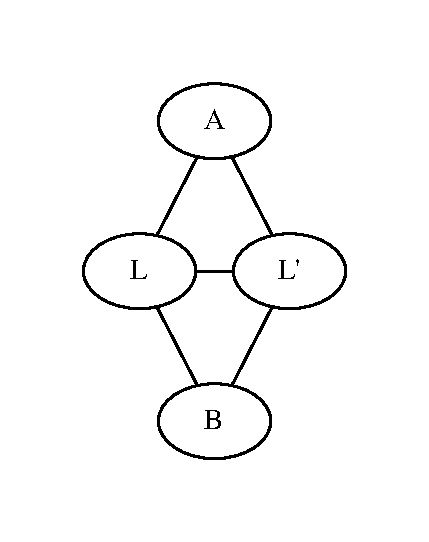
\includegraphics[width=0.3\textwidth]{img/intersectiongraph.pdf}
\label{graph}
\caption{depiction of a contradicting diamond }
\end{figure}
On the other hand the existence of such adjacent triangles contradicts lemma \ref{lemmaCoplanarLinesOnCubic}.
We will use this argument several times, so let's give it a name. We call a configuration like in figure \ref{graph} a \emph{contradicting diamond}.

Now let $L,M$ be disjoint lines on $S$.
These exist: For some line $L' \subset S$ we can choose $L := \Lambda^1(L')$ and $M := \Lambda^2(L')$, so $L \boxtimes L', M \boxtimes L'$.
Suppose $L\boxtimes M$, then $L,M,L'$ are coplanar, but so are $L,L',V^1(L')$ which gives us the contradicting diamond $L,L',V^1(L'),M$.
We conclude
\begin{equation*}
L\square M
\end{equation*}

The next observation is that either $M\boxtimes \Lambda^i(L)$ or $M\boxtimes V^i(L)$ for each $i=1,..5$.
This is because $M$ intersects the hyperplane $\Pi^i(L)$ (by corollary \ref{corollarySimpleIntersect}), $M \subset S - L$ and $S \cap \Pi^i(L) = \Lambda^i(L) \cup V^i(L) \cup L$. Therefore this lemma holds:
\begin{lemma} \label{lemmaBinaryIntersection}
If $N\square L$ are lines on $S$, then either $N \boxtimes \Lambda^i(L)$ or $N \boxtimes V^i(L)$.
If $N\boxtimes L$, then $N$ can furthermore meet $\Lambda^i(L)\cap V^i(L)$.
\end{lemma}

Assume without loss of generality that $\Lambda^i(L) = \Lambda^i(M) =: L_i$. With this notation we have
\begin{lemma} \label{lemmaCrosswiseIntersection}
$V^i(L) \boxtimes V^j(M)$ iff $i \neq j$.
\end{lemma}
\begin{proof}
We just apply the lemma \ref{lemmaBinaryIntersection}.
Let $i \in\{ 1,..5\}$.
Suppose $V^i(L) \boxtimes V^i(M)$, then $V^i(L),V^i(M),L_i$ are coplanar and $M,V^i(M),L_i$ are coplanar, earning us a contradicting diamond.
Now let $j \neq i$.
Assume $V^i(L) \boxtimes L_j$.
Then $L,M,L_j$ being coplanar and $L,L_j,V^i(L)$ being coplanar implies that $L,L_j,M,V^i(L)$ is a contradicting diamond.
Therefore $V^i(L) \boxtimes V^j(M)$, due to lemma \ref{lemmaBinaryIntersection}.
\end{proof}

So far we found 17 lines $L,M,\Lambda^i(L),V^i(L),V^i(M)$.
The other ten are obtained via the following lemma.

\begin{lemma}
There is a bijection between the 3-element subsets of $\{\Lambda^1(L),..\Lambda^5(L)\}$ and the remaining lines on $S$ which are not among the 17 already accounted for.
\end{lemma}

This implies that precisely $\binom{5}{3} = 10$ more lines exist, for a total of 27.

\begin{proof}
Let $N$ be a line on $S$ other than the 17 from before.
We show that $N$ intersects precisely three of $\Lambda^i(L)$ by showing that the other cases are not possible.
\paragraph{Case 1: \textnormal{$N$ intersects $\geq 4$ of the $L_i$.}}
In that case the four disjoint lines have transversals $L,M,N$.
This is only possible if the four lines lie on a quadric surface (by corollary \ref{corollaryCubicContainsQuadric}), contradiction.
\paragraph{Case 2: \textnormal{$N$ intersects $\leq 2$ of the $L_i$.}}
Without loss we can assume $N$ to meet either one of these sets of five disjoint lines:
\begin{itemize}
\item $V^1(L) ,V^2(L) ,V^3(L) ,V^4(L) ,V^5(L)$.
\item $L_1,V^2(L),V^3(L) ,V^4(L) ,V^5(L)$.
\item $L_1, L_2, V^3(L) ,V^4(L) ,V^5(L)$.
\end{itemize}
So we assume one of these sets to have $N$ as common transversal, as well as $V^1(M) $ and $L$ by default.
This leads to a contradiction just like in the first case.

This shows that the following function is well-defined:
\begin{align*}
\kappa : \left\lbrace\text{remaining lines}\right\rbrace \to &\left\lbrace \text{3-element subsets of }\{L_1,..L_5\}\right\rbrace \\
N \mapsto &\mkset{ L_i}{N\boxtimes L_i}
\end{align*}

We show injectivity: Suppose the lines $N$ and $N'$ meet the same lines $L_i$. Then $N$ meets some $V^j(M)$ and some $V^k(L)$ ($j \neq k$), same for $N'$.
By lemma \ref{lemmaCrosswiseIntersection}, $V^j(M) \boxtimes V^k(L)$.
If $N\neq N'$ we obtain a contradicting diamond $N,N',V^j(M),V^k(L)$, so $N=N'$, proving injectivity.

Let's fix one $L_i$.
We know that $L_i$ meets ten lines by corollary \ref{corollaryFivePlanes}.
Four of these have been counted: $M,V^i(M),L,V^i(L)$.
As we have just seen, the missing six meet two out of the four lines $\{ L_j \}_{j\neq i}$, so there are $\binom{4}{2}$ possibilities to choose such two.
By injectivity of $\kappa$ all these possibilities must be exhausted, hence $\kappa$ is also surjective and we're done with the proof.
\end{proof}
